\documentclass[12pt,mathserif]{beamer}

\usepackage{etex, amssymb, amsmath, amsfonts, bm, algorithmic, algorithm, multirow, array, graphicx, epstopdf, wrapfig, empheq, fancybox, tikz, color, url, hyperref, subfigure, soul, ragged2e, pgfplots, ulem, xcolor, colortbl, filecontents, diagbox, setspace}

\usepackage{amsmath, amsfonts, amssymb,graphicx,xcolor}

\usepackage{pgfplots}

\usetikzlibrary{shapes.arrows,snakes,mindmap,trees,backgrounds,decorations.footprints,calc}

\usetheme{Warsaw}

\setbeamertemplate{footline}
{
  \leavevmode%
  \hbox{%
  \begin{beamercolorbox}[wd=.4\paperwidth,ht=2.25ex,dp=1ex,center]{author in head/foot}%
    \usebeamerfont{author in head/foot}R. Oliynykov, I. Gorbenko, O. Kazymyrov, et al.
  \end{beamercolorbox}%

  \begin{beamercolorbox}[wd=.6\paperwidth,ht=2.25ex,dp=1ex,right]{date in head/foot}%
    \usebeamerfont{date in head/foot}
    \insertshorttitle{}\hspace*{3em}
    \insertframenumber{} / \inserttotalframenumber\hspace*{2ex} 
  \end{beamercolorbox}
  }%

  \vskip0pt%

}

\makeatother


\setbeamertemplate{headline}{}


\setbeamertemplate{headline}{}

\newcolumntype{g}{>{\columncolor{green!20}}c}
\newcolumntype{C}[1]{>{\centering\let\newline\\\arraybackslash\hspace{0pt}}m{#1}}
%\newcommand{\bigcell}[2]{\begin{tabular}{@{}#1@{}}#2\end{tabular}}
%\newtheorem{proposition}{Proposition}
%\DeclareMathOperator{\F}{\mathbb{F}}
%\DeclareMathOperator{\tr}{tr}

%\title[A New Encryption Standard of Ukraine: The Block Cipher "Kalyna"]{A New Encryption Standard of Ukraine:\\ The Block Cipher "Kalyna" (DSTU~7624:2014)}

\title[A New Standard of Ukraine: The Block Cipher "Kalyna"]{A New Encryption Standard of Ukraine:\\ The Block Cipher "Kalyna" (DSTU~7624:2014)}

\author
{
	Roman Oliynykov,\\ Ivan Gorbenko, Oleksandr Kazymyrov, Victor Ruzhentsev, Yurii Gorbenko and Viktor Dolgov
}

\institute{
JSC Institute of Information Technologies, \\ V.N.Karazin Kharkiv National University,\\ Kharkiv National University of Radio Electronics\\ 
Ukraine\\
\texttt{roliynykov@gmail.com}
}


\date{\scriptsize{July 8th, 2015\\Central European Conference on Cryptology\\Klagenfurt, Austria} }

\begin{document}
 	\begin{frame}
		\maketitle
	\end{frame}
  
	\begin{frame}
    		\frametitle{Outline}
    		\begin{itemize}
    			\item The block cipher GOST 28147-89 and its replacements in post-Soviet countries
    			\item The new Ukrainian block cipher "Kalyna" \hfill \\
    			\begin{itemize}
				\item General structure    				
    				\item Component properties
    				\item Key schedule
    				\item Cryptographic strength
    			\end{itemize}
    			\item Performance comparison with other ciphers
    			\item Other components of the Ukrainian national standard DSTU 7624:2014
    			\item Conclusions
    		\end{itemize}
  	\end{frame}
  	
	\begin{frame}{Block cipher GOST 28147-89}
		\textcolor{blue}{Advantages}
			\begin{itemize}
				\item a well known and researched cipher, adopted as national standard in 1990 
				\item acceptable encryption speed (cf.TripleDES) 
				\item appropriate for lightweight cryptography
				\item good S-boxes provide practical strength
			\end{itemize}
		\textcolor{blue}{Disadvantages}
			\begin{itemize}
				\item theoretically broken
				\item huge classes of weak keys
				\item special S-boxes (non-bijective) allows practical ciphertext-only attacks
				\item encryption speed significantly slower in comparison to modern block ciphers like AES
			\end{itemize}
		\begin{spacing}{0.5}
		\begin{tiny}
  		 GOST 28147-89 is withdrawn in Belarussia (legacy-only application) and will be replaced in Russia (will remain as additional 64-bit algorithm); GOST 28147-89 was refused to be included to ISO/IEC 18033-3
  		\end{tiny}
  		\end{spacing}
	\end{frame}	
	
 
	\begin{frame}
		\frametitle {Replacements for GOST 28147-89 in Belarussia}
%		\begin{description}
%			\item[Belarussia: STB 34.101.31-2011 (BelT)] \hfill \\
			\textcolor{blue}{Belarussia: STB 34.101.31-2011 (BelT)}
			\begin{itemize}
				\item block length is 128 bits; key length is 128, 192 or 256 bits
				\item 8-rounds Feistel network with Lai-Massey scheme
				\item a single byte S-box with good cryptographic properties
				\item no key schedule like in GOST (encryption key shorter than 256 bits is padded by zeros)
				\item no cryptanalytical attacks better than exhaustive search are known
				\item faster than GOST, slower than AES
			\end{itemize}
%		\end{description}				
		
	\end{frame}
 
	\begin{frame}
%	\frame[shrink] {
		\frametitle {Replacements for GOST 28147-89 in Russia}
%		\begin{description}%[leftmargin=-.5in]
%			\item[Russia: draft standard "Kuznyechik" ("Grasshopper")] \hfill \\
%			\leftmargini=.2in
			\textcolor{blue}{Russia: draft standard "Kuznyechik" ("Grasshopper")}
			\begin{itemize}%[leftmargin=-.5in]
				%\setlength{\itemindent}{-.9in}
				%\leftmargin=-0.9in			
				\item block length is 128 bits; key length is 256 bits
				\item 9 rounds of Rijndael-like transformation
				\item single byte S-box (common with the new Russian hash GOST 34.11-2012 "Stribog")
				\item non-circulant MDS matrix of 16x16 size over $GF(2^8)$ (different from that in "Stribog")
				\item key schedule based on a Feistel network and involves round transformation (like in CS-cipher)
				\item no cryptanalytical attacks faster than exhaustive search are known
				\item faster than GOST, slower than AES
			\end{itemize}
%		\end{description}				
%	}
		\begin{tiny}
			GOST 28147-89 will be used as an additional legacy cipher in the new Russian standard
		\end{tiny}
		
	\end{frame}

%	\begin{frame}
	\frame[shrink] {
		\frametitle{Block cipher "Kalyna"}
		
		\begin{itemize}
			\item normal, high and ultra high security level (block and key length 128, 256 and 512 bits)
			\item transparent construction and conservative design
			\item Rijndael-like SPN structure
			\item four different S-boxes (not CCZ-equivalent) with optimized cryptographic properties 
			\item 8x8 MDS matrix over $GF(2^8)$
			\item one set of look-up tables for ECB encryption in software implementation (better performance of encryption and decryption for CTR, CFB, CMAC, OFB, GCM, GMAC, CCM modes of operation)
%			\item common look-up tables with the new Ukrainian hash function "Kupyna" (DSTU 7564:2014)
			\item a new construction of key schedule based on the round function
			\item effective in software and software-hardware implementations, common look-up tables with the hash function "Kupyna" (DSTU 7564:2014) 
		\end{itemize}
	}
%	\end{frame}
  
	\begin{frame}
		\frametitle{"Kalyna": supported block and key length  }
			
		\begin{table}
			 \begin{center}
			  \begin{tabular}{ | c | c | c | c | }
			    \hline
			    \# & Block size (\textit{l}) & Key length (\textit{k}) & Rounds (\textit{t}) \\ \hline \hline
				 1 & \multirow{2}*{128} & 128 & 10 \\ %\cline{1-1}\cline{3-4}
				 2 &     & 256 & 14    \\ \hline
			     3 & \multirow{2}*{256} & 256 & 14 \\ %\cline{1-1}\cline{3-4}
			     4 &     & 512 & 18   \\ \hline
			     5 & 512 & 512 & 18  \\
			    \hline
			  \end{tabular}
			 \end{center} 
			\end{table}
	
	\end{frame}
	
	\begin{frame}
		\frametitle{Block cipher "Kalyna": structure}

	    \begin{center}
				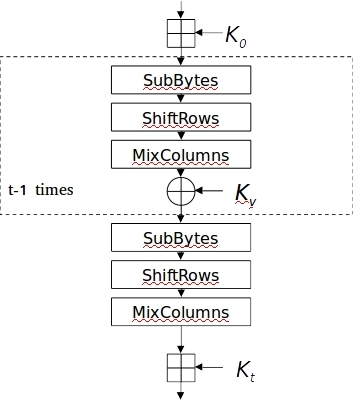
\includegraphics[width=0.4\textwidth]{./pics/structure.jpg}    
		\end{center}			

		\begin{equation*}
T_{l,k}^{(K)} = \eta_l^{(K_t)} \circ \psi_l \circ \tau_l \circ \pi_l ' \circ \prod_{\nu=1}^{t-1} 			(\kappa_l^{(K_\nu)} \circ \psi_l \circ \tau_l \circ \pi_l ' ) \circ \eta_l^{(K_0)} 		
		\end{equation*}
		
	\end{frame}

	\begin{frame}
		\frametitle{"Kalyna": characteristics of S-boxes}	
		
		\begin{table}
			 \begin{center}
			  \begin{tabular}{ | c | c | c | c | c | }
			    \hline
			     \multirow{2}*{ Characteristic } & \multicolumn{4}{c|}{ S-box } \\ \cline{2-5}
			      & 1 & 2 & 3 & 4 \\ \hline
			      Non-linearity of Boolean functions & \multicolumn{4}{c|}{ 104 } \\ \hline
			      Min. algebraic degree of Boolean functions & \multicolumn{4}{c|}{ 7 } \\ \hline
			      Max. value of difference distribution table & \multicolumn{4}{c|}{ 8 } \\ \hline
			      Max. value of linear approximation table & \multicolumn{4}{c|}{ 24 } \\ \hline
			      Overdefined system degree & \multicolumn{4}{c|}{ 3 } \\ \hline
			      Number of cycles & 4 & 4 & 6 & 4 \\ \hline
			      Minimal cycle length & 6 & 8 & 4 & 4 \\ \hline
			  \end{tabular}
			 \end{center} 
			\end{table}
			
			\begin{scriptsize}
			Non-linearity is the best known for S-boxes with $3^{rd}$ degree of overdefined system (the highest among S-boxes of Crypton, Safer+, Skipjack, SNOW, Twofish, Whirlpool, СS, Anubis, Stribog/Kuznyechik, STB)
			\end{scriptsize}
	
	\end{frame}
	
	\begin{frame}
		\frametitle{"Kalyna" ShiftRows: 128,256 and 512-bit block}
		
		\begin{columns}[c]
			\begin{column}{.48\textwidth}
				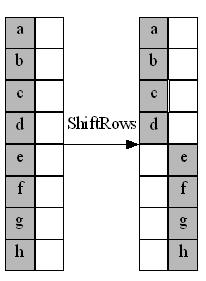
\includegraphics[scale=0.45]{./pics/shift128.jpg}
			\end{column}

			\begin{column}{.48\textwidth}
				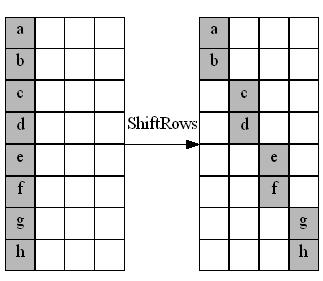
\includegraphics[scale=0.45]{./pics/shift256.jpg}
			\end{column}

		\end{columns}		

		\begin{center}
			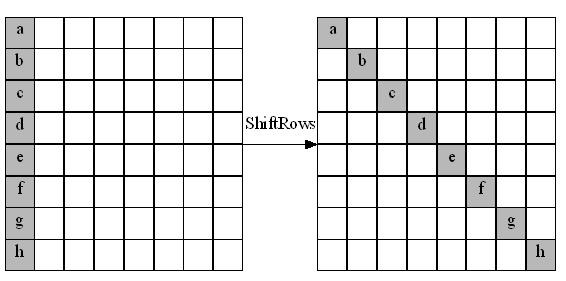
\includegraphics[scale=0.45]{./pics/shift512.jpg}
		\end{center}
		
		
	\end{frame}
	
	
	\begin{frame}
		\frametitle{Linear transformation of "Kalyna": MDS matrix}

	    \begin{center}
				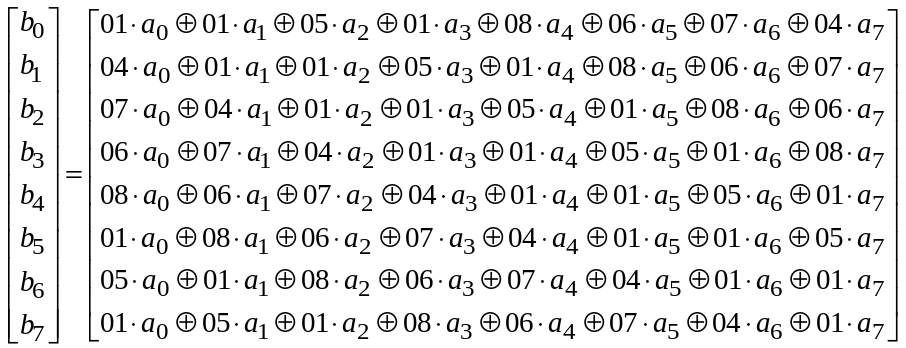
\includegraphics[scale=0.35]{./pics/kalyna-mds.jpg}    
		\end{center}			

%		\begin{scriptsize}
%			Maximal branch number ($B_n=9$)
%		\end{scriptsize}


	\end{frame}	
	
	\begin{frame}
		\frametitle {Requirements to "Kalyna" key schedule}
		
		\begin{itemize}
			\item each round key depends non-linear on each encryption key bit 
			non-linear dependence of each round key bit on each encryption key bit
			\item protection from cryptanalytic attacks aimed to key schedule
			\item high computation complexity of obtaining encryption key having one or several round keys (one-way transformation, additional protection from side-channel attacks)
			\item key agility is less than three
			\item possibility to generate round keys in direct and reverse order
			\item implementation simplicity (application of transformations from the round function only)
		\end{itemize}
	\end{frame}

	\begin{frame}
		\frametitle {"Kalyna" key schedule}
		
		\begin{columns}[c]
			\begin{column}{.60\textwidth}
				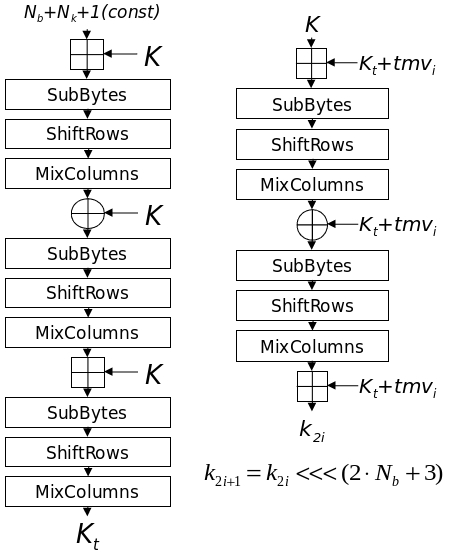
\includegraphics[width=0.8\textwidth]{./pics/kalyna-key-schedule.jpg}
			\end{column}

			\begin{column}{.36\textwidth}

				\begin{scriptsize}
				
				$tmv_0 = 0x01000100..0100$
				$tmv_{i+2} = tmv_i << 1$
				
				\end{scriptsize}
				
			\end{column}

		\end{columns}		
		
			
%	    \begin{center}
%				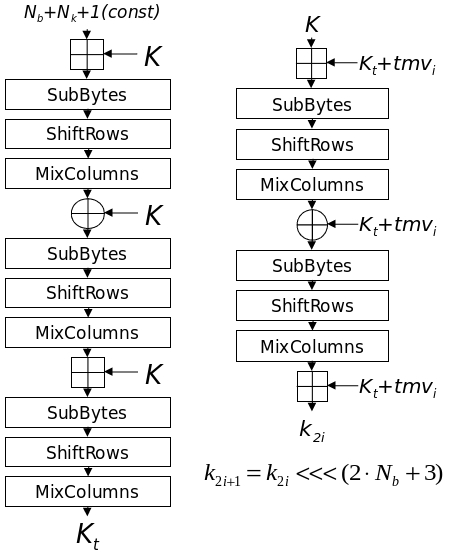
\includegraphics[width=0.4\textwidth]{./pics/kalyna-key-schedule.jpg}    
%		\end{center}			

		\begin{scriptsize}
		
			\begin{equation*}
\Theta^{(K)}=\psi_l \circ \tau_l \circ \pi_l ' \circ \eta^{(K_\alpha)}_l \circ
\psi_l \circ \tau_l \circ \pi_l ' \circ \kappa^{(K_\omega)}_l \circ
\psi_l \circ \tau_l \circ \pi_l ' \circ \eta^{(K_\alpha)}_l 
			\end{equation*}				

			\begin{equation*}
\Xi^{(K, K_\sigma, i)}= \eta^{(\varphi_i (K_\sigma) )}_l \circ 
\psi_l \circ \tau_l \circ \pi_l ' \circ
\kappa^{(\varphi_i (K_\sigma) )}_l \circ 
\psi_l \circ \tau_l \circ \pi_l ' \circ \eta^{(\varphi_i (K_\sigma) )}_l 
			\end{equation*}				

	\end{scriptsize}
	
	\end{frame}
	
	\begin{frame}
		\frametitle{Cryptographic strength of "Kalyna"}
		Block cipher provides strength to considered methods of cryptanalysis:
		\begin{itemize}
			\item for 128-bit block: after 5\textsuperscript{th} round (out of 10 or 14, depending on the key length)
			\item for 256-bit block: after 6\textsuperscript{th} round (out of 14 or 18)
			\item for 512-bit block: after 8\textsuperscript{th} round (out of 18)
		\end{itemize}
	\end{frame}
	
	\begin{frame}
		\frametitle {"Kalyna" performance comparison with other block ciphers}
		\framesubtitle{(Intel Core i5, 64-bit Linux, gcc v4.9.2, best compiler optimization)}
		
		\begin{center}
			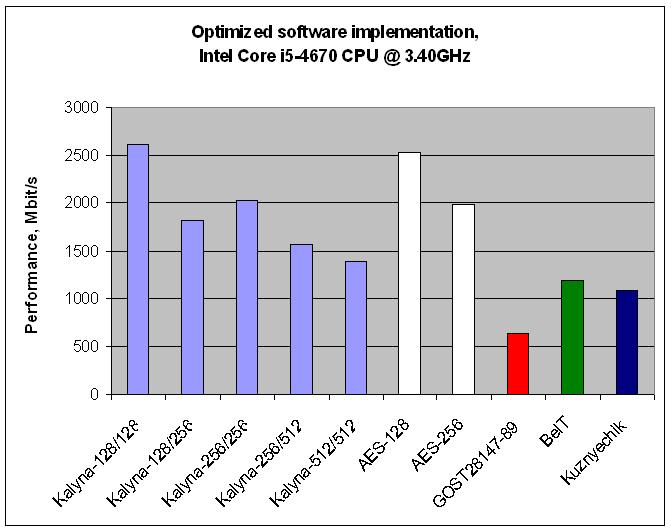
\includegraphics[scale=0.4]{./pics/performance_core_i5.jpg}
			
			\begin{tiny}
				https://github.com/Roman-Oliynykov/ciphers-speed/
			\end{tiny}
		
		\end{center}
	
	\end{frame}		
	
	\begin{frame}
		\frametitle {"Kalyna" performance comparison with other block ciphers}
		\framesubtitle{(Intel Core i5, 64-bit Linux, gcc v4.9.2, best compiler optimization)}
		
		\begin{table}
			 \begin{center}
			  \begin{tabular}{ | c | c | c | }
			    \hline
			    \# & Block cipher & Performance, Mbit/s \\ \hline
			    1 & Kalyna-128/128 & 2611.77 \\ \hline
				2 & Kalyna-128/256 &	1809.70 \\ \hline
				3 & Kalyna-256/256 &	2017.97 \\ \hline
				4 & Kalyna-256/512 &	1560.89 \\ \hline
				5 & Kalyna-512/512 &	1386.46 \\ \hline
				6 & AES-128 & 2525.89 \\ \hline
				7 & AES-256 & 1993.53 \\ \hline
				8 & GOST 28147-89 &	639.18 \\ \hline
				9 & STB 34.101.31-2011 (BelT) & 1188.83 \\ \hline
				10 & Kuznyechik & 1081.08 \\ \hline
			  \end{tabular}
			 \end{center} 
			\end{table}
		
	\end{frame}

	\begin{frame}
		\frametitle {"Kalyna" performance comparison with other block ciphers}
		\framesubtitle{(iMac 13.2, Intel Core i7, best compiler optimization)}
		
		\begin{center}
			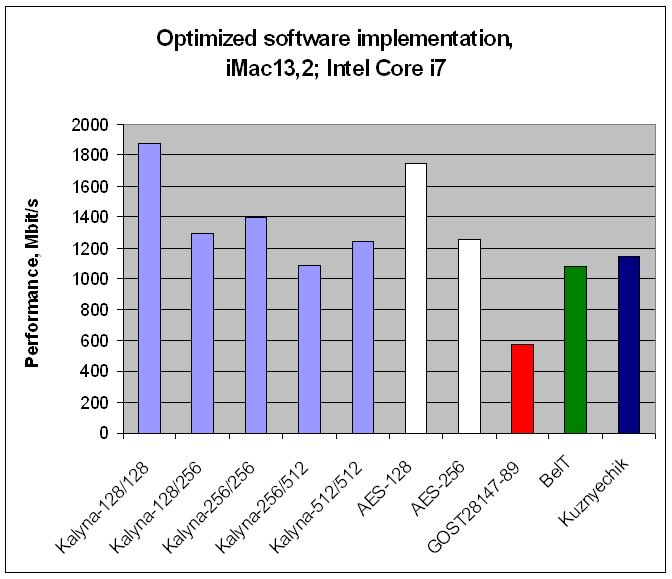
\includegraphics[scale=0.4]{./pics/performance_core_iMac.jpg}
			
			\begin{tiny}
				https://github.com/Roman-Oliynykov/ciphers-speed/
			\end{tiny}
		
		\end{center}
	
	\end{frame}		
	
	\begin{frame}
		\frametitle {"Kalyna" performance comparison with other block ciphers}
		\framesubtitle{(iMac 13.2, Intel Core i7, best compiler optimization)}
		
		\begin{table}
			 \begin{center}
			  \begin{tabular}{ | c | c | c | }
			    \hline
			    \# & Block cipher & Performance, Mbit/s \\ \hline
			    1 & Kalyna-128/128 &	 1874.39 \\ \hline
				2 & Kalyna-128/256 &	 1295.55 \\ \hline
				3 & Kalyna-256/256 &	 1392.48 \\ \hline
				4 & Kalyna-256/512 &	 1088.88 \\ \hline
				5 & Kalyna-512/512 &	 1243.49 \\ \hline
				6 & AES-128 & 1747.09 \\ \hline
				7 & AES-256 & 1257.43 \\ \hline
				8 & GOST 28147-89 &	576.10 \\ \hline
				9 & STB 34.101.31-2011 (BelT) & 1080.02 \\ \hline
				10 & Kuznyechik & 1146.31 \\ \hline
			  \end{tabular}
			 \end{center} 
			\end{table}
		
	\end{frame}
	
%	\begin{frame}
	\frame[shrink] {
		\frametitle {DSTU 7624:2014 also includes}
		
		\begin{itemize}
			\item Ten modes of operation for the new block cipher \hfill \\
				\begin{itemize}
					\item ISO 10116: ECB, CBC, CFB, OFB, CTR
					\item additional modes, simplified/improved comparing to NIST SP 800-38: GCM/GMAC (securing IP-traffic), CCM (confidentiality \& integrity), XTS (on-the-fly encryption of information storage), KW (key data protection)
				\end{itemize}
			\item Test vectors (including not aligned to the block length and, for some modes, byte length)
			\item Requirements to implementation: \hfill \\ 
				\begin{itemize}
					\item general concepts paying developer's attention to take steps for prevention of side-channel attacks, timing attacks, CRIME/BREACH specific vulnerabilities, etc.
					\item limits on the total number of invocation of the block cipher during the encryption key lifetime
					\item message replay prevention
				\end{itemize}
			\item etc.
		\end{itemize}
	}
%	\end{frame}

	\begin{frame}
		\frametitle {Conclusions}
		\framesubtitle {	The new block cipher "Kalyna" provides}
		
		\begin{itemize}
			\item normal, high and ultra high security level
			\item transparent construction and conservative design
			\item fast and effective software and software-hardware implementations on modern 64-bit platforms
			\item optimized construction for better performance on encryption and
decryption for CTR, CFB, CMAC, OFB, GCM, GMAC, CCM modes of operation 
			\item new construction of key schedule based on the round
transformation
			\item common look-up tables with the hash
function "Kupyna" (the new Ukrainian standard DSTU 7564:2014)
		\end{itemize}
		
		\begin{scriptsize}
			\begin{spacing}{0.5}
			Besides the block cipher, the new Ukrainian standard DSTU 7624:2014 defines ten modes of operation, test vectors, requirements for implementation, limits on protected information amount for a single key application, etc.	
			\end{spacing}
		\end{scriptsize}
	\end{frame}

	
 
\end{document}

